\chapter{Scénario de déploiement}
\label{sec:deploiement}

%%%%%%%%%%%%%%%%%
%%% Prototype %%%
%%%%%%%%%%%%%%%%%
\section{Test du prototype}
    \paragraph{} Pour compléter les tests de portée que nous avons réalisé, nous pouvons réaliser divers essais. Tout d'abord, nous pouvons essayer de vérifier le taux moyen d'intégrité des données. Nous pouvons également voir si les modules peuvent communiquer entre eux à travers différents types de matériaux (s'intéresser à la traversée des murs par exemple). Il peut être intéressant de faire des tests d'autonomie également et tester l'efficacité des différents mode de gestion de l'énergie.\\
    Pour les capteurs, il est nécessaire de tester leur fiabilité et voir s'ils renvoient des données cohérentes. Leur impact sur la batterie est aussi intéressant à mesurer.



%%%%%%%%%%%%%%%%%%%
%%% Déploiement %%%
%%%%%%%%%%%%%%%%%%%
\section{Déploiement}
    \begin{figure}[h]
        \centering
        \begin{tikzpicture}
    % Réduit l'interligne
    \linespread{0.7}
    
    % Inclus l'image
    \node[anchor=south west,inner sep=0] (image) at (0,0) {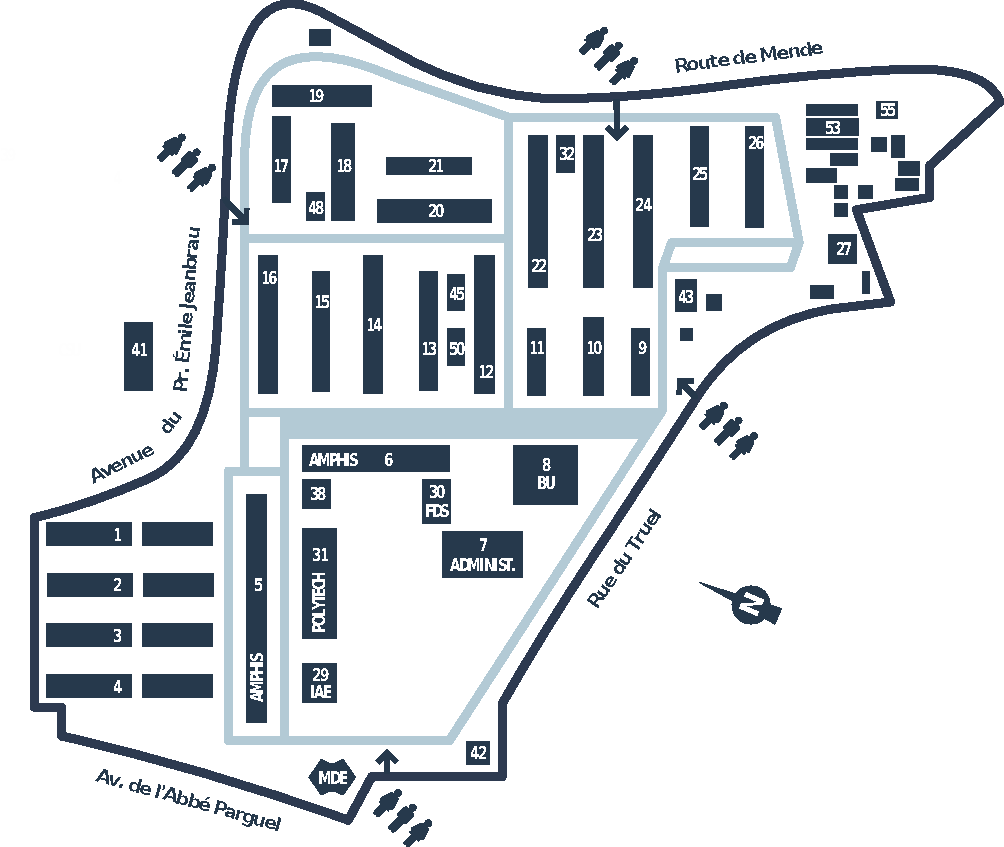
\includegraphics[trim={9.4cm 9cm 0cm 0cm},clip,scale=1.3]{images/plan.pdf}};
    
    % Définitition des styles
    \tikzstyle{wasp}        = [black]
    \tikzstyle{waspRelais}  = [wasp,fill=blue]
    \tikzstyle{waspCapt}    = [wasp,fill=yellow]
    \tikzstyle{waspBoth}    = [wasp,fill=OliveGreen]
    \tikzstyle{conn}        = [OliveGreen,ultra thick,dotted]
    \tikzstyle{bat}         = [red,ultra thick]
    \tikzstyle{legend}      = [anchor=west,text=darkgray]
    \tikzstyle{onMap}       = [anchor=center,text=red,text width=2.5cm,align=center]

    % Zone de dessin
    \begin{scope}[x={(image.south east)},y={(image.north west)}]
        % Grille
        %\draw[help lines,xstep=.05,ystep=.1] (0,0) grid (1,1);
        
        % Repère
        %\foreach \x in {0,1,...,9} { \node [anchor=north] at (\x/10,0) {0.\x}; }
        %\foreach \y in {0,1,...,9} { \node [anchor=east] at (0,\y/10) {0.\y}; }
        
        % Animalerie
        \draw[bat,rounded corners] (0.55,0.51) rectangle (0.688,0.68);
        \node[onMap] at (0.63,0.72) {Animalerie};
        
        % Bâtiment de recherche
        \draw[bat,rounded corners] (0.166,0.08) rectangle (0.225,0.58);
        \node[onMap] at (0.17,0.042) {Bâtiment de recherche};
        
        % Connections
        \draw[conn] (0.445,0.500)  --  (0.322,0.5);     % R3 -- R2
        \draw[conn] (0.322,0.500)  --  (0.198,0.5);     % R2 -- R1
        \draw[conn] (0.578,0.595)  --  (0.445,0.5);     % R3 -- M
        \draw[conn] (0.620,0.650)  --  (0.578,0.595);   % C1 -- M
        \draw[conn] (0.620,0.542)  --  (0.578,0.595);   % C3 -- M
        \draw[conn] (0.660,0.595)  --  (0.578,0.595);   % C2 -- M

        % Waspmotes
        \draw[waspRelais] (0.445,0.500)  circle  (0.14cm);  % R3
        \draw[waspRelais] (0.322,0.500)  circle  (0.14cm);  % R2
        \draw[waspRelais] (0.198,0.500)  circle  (0.14cm);  % R1
        \draw[waspCapt]   (0.620,0.650)  circle  (0.14cm);  % C1
        \draw[waspCapt]   (0.620,0.542)  circle  (0.14cm);  % C3
        \draw[waspCapt]   (0.660,0.595)  circle  (0.14cm);  % C2
        \draw[waspBoth]   (0.578,0.595)  circle  (0.14cm);  % M

        % Légende
        \footnotesize
        \draw[darkgray] (0.775,-0.02) rectangle (1.15,0.32);
        \node[anchor=center,text=darkgray] at   (0.91,0.28) {\bfseries\underline{\textit{Légende}}};
        \draw[waspRelais]    (0.80,0.22) circle (0.14cm);
        \node[legend] at     (0.82,0.22) {Waspmote relais};
        \draw[waspCapt]      (0.80,0.17) circle (0.14cm);
        \node[legend] at     (0.82,0.17) {Waspmote capteur};
        \draw[waspBoth]      (0.80,0.12) circle (0.14cm);
        \node[legend] at     (0.82,0.12) {Waspmote mère};
        \draw[conn]          (0.785,0.07) -- (0.815,0.07);
        \node[legend] at     (0.82,0.07) {Connexion};
        \draw[bat,thick]     (0.785,0.005) rectangle (0.815,0.035);
        \node[legend] at     (0.82,0.020) {Bâtiment clef};
    \end{scope}
\end{tikzpicture}
        \caption{Plan d'installation}
        \label{fig:install}
    \end{figure}

    \paragraph{} La figure \ref{fig:install} décrit notre scénario de déploiement. L'objectif consiste à installer une ou plusieurs Waspmote(s) bardée(s) de capteurs par salle, une Wasmote mère ou centrale qui recueillera les données de ces autres Waspmotes, et puis enfin plusieurs Waspmotes relais jusqu'au bâtiment 24 qui serviront à faire transiter les données jusqu'à ce bâtiment. L'installation nécessite plus de Waspmotes qu'indiquer dans le plan, la portée du Zigbee n'étant pas suffisante pour sauter de bâtiment en bâtiment. 
    
    \paragraph{} Nous avons également un autre scénario subsidiaire où la Waspmote mère comporterait un module 3G et communiquerait au serveur les données reçues directement par internet via sa connexion mobile. Cette option nécessite néanmoins de tester l'autonomie d'une Wasmpote utilisant une connexion 3G et oblige à la souscription d'un abonnement 3G auprès d'un opérateur mobile. 
    
    \paragraph{} Enfin, un dernier scénario tertiaire serait de mélanger des modules Zigbee et des modules LoRaWAN. Les Waspmotes avec les capteurs communiqueraient en Zigbee avec la Waspmote mère. Sur celle-ci serait branché un module LoRaWAN en plus du module Zigbee\footnote{Les Waspmotes peuvent supporter jusqu'à deux modules de communication en même temps.}. Une dernière Waspmote serait positionnée au niveau du bâtiment 24 avec un module LoRaWAN. Si la portée de LoRaWAN est dans les faits aussi élevée que ce que les ressources Internet nous disent, alors il ne devrait y avoir aucun souci pour que la Waspmote mère communique avec la Waspmote du bâtiment 24 sans installer de Waspmotes relais. 



%%%%%%%%%%%%%%%%%
%%% Autonomie %%%
%%%%%%%%%%%%%%%%%
\section{Optimisation de l'autonomie des Waspmotes}
    \paragraph{} Avant de parler du travail d'optimisation de l'autonomie, il est nécessaire d'introduire les différentes interruptions qui peuvent être reçues par le microcontrôleur de la Waspmote :

    \begin{itemize}
        \item \textbf{Les interruptions synchrones} sont programmées par le développeur. Elles correspondantes à des minuteurs qui peuvent être soit périodiques, par exemple une alarme toutes les 10 secondes ou tous les premiers lundis du mois, soit relatifs, par exemple une alarme programmée pour durer 10 minutes à partir d'un moment donné.
        \item \textbf{Les interruptions asynchrones} proviennent des capteurs. Une alarme peut être déclenchée quand un capteur a atteint une certaine valeur. Elles peuvent également provenir de l'accéléromètre qui en fonction du mouvement de la Waspmote peut envoyer un signal (en cas de chute par exemple).
    \end{itemize}

    \paragraph{} Au microcontrôleur est associé un << Watchdog >> ou chien de garde en français, qui est une sorte de RTC intégrée et qui compte les cycles d'horloge. Il peut être utilisé à intervalles de temps réguliers. Ces intervalles peuvent prendre les valeurs suivantes : 16ms, 32ms, 64ms, 128ms, 256ms, 500ms, 1s, 2s, 4s, 8s. Au delà de 8s, c'est le RTC qui prend le relais.

    \begin{table}[h]
        \centering
        \begin{tabular}{l | l}
            \bfseries{Mode}     & \bfseries{Consommation}\tabularnewline\hline
            En marche           & 15~mA\tabularnewline
            Veille              & 55~µA\tabularnewline
            Veille prolongée    & 55~µA\tabularnewline
            Hibernation         & 0.07~µA
        \end{tabular}
        \caption{Consommation en fonction des différents états du Waspmote}
        \label{tab:conso}
    \end{table}
    
    \paragraph{} Les différentes interruptions et le chien de garde permettent d'expliquer  la gestion de l'énergie des Waspmotes. Quatre types de mode de gestion de l'énergie se distinguent dans la \textit{figure \ref{tab:conso}} :
    
    \begin{enumerate}
        \item \textbf{Mode en marche :} fonctionnement normal du Waspmote.
        \item \textbf{Mode veille :} le microcontrôleur est placé dans un état latent, toutes les interruptions asynchrones le sortent de cet état ainsi que les interruptions synchrones venant du chien de garde. Les cycles de sommeil en mode veille peuvent durer de 32ms à 8s (ou plus mais il y a alors tout intérêt à passer en mode veille prolongée ou hibernation).
        
        \item \textbf{Mode veille prolongée :} similaire au mode veille, à part pour les interruptions synchrones qui ne réveillent le microcontrôleur qu'en cas d'alarme RTC. Cycle compris entre 1s et plusieurs jours/mois/années.
        
        \item \textbf{Mode hibernation :} extinction de toute la Waspmote hormis l'horloge RTC. Seuls des interruptions synchrones RTC peuvent réveiller le microcontrôleur. Cycle compris entre 1s et plusieurs jours/mois/années. La consommation est réduite à son minimum.
    \end{enumerate}
    
    \paragraph{}Chaque module présentent aussi quatre modes d'énergie: modes marche, en veille, hibernation et éteint. Les modes veille et hibernation sont programmés par les fabricants et sont donc spécifiques à chaque module (voir la doc du module). Le mode éteint a été développé par Libelium et permet comme son nom l'indique d'éteindre les modules en outre-passant les programmes des fabricants et permet d'atteindre une consommation quasi-nulle.
    
    \paragraph{}Il est difficile de définir avec justesse la consommation de la Waspmote en incluant les capteurs. Ceux-ci sont de diverses natures et la documentation ne fournit pas d'information sur la consommation des capteurs. Elle indique néanmoins que chaque capteur peut avoir pour tension +3.3V/+5V et une intensité maximale égale à 200~mA.
    
    \paragraph{}Cependant, il est possible d'établir un scénario assez simple reflétant le fonctionnement de notre application. On peut imaginer le cas d'utilisation suivant : la Waspmote dispose d'un capteur de température, d'humidité et de luminosité. Toutes les heures, la Waspmote envoie au serveur les données relevées par les capteurs. Ces relevés peuvent durer plusieurs secondes pour avoir plusieurs valeurs, permettant de faire une moyenne et de supprimer les valeurs non cohérentes (parasites). Une fois l'envoi réalisé, la Waspmote se met en mode hibernation et ne se réveillera qu'à la prochaine heure.
    
    \paragraph{}En cas d'échec de l'envoie, les données sont gardées et la Waspmote tentent de les envoyer toutes les secondes par exemple. Entre chaque tentative, elle passe en mode veille. En cas d'échec prolongé, la Waspmote se met en veille prolongée ou hibernation pour une durée plus longue (par exemple 1h). Elle essaie alors de transmettre de nouveau les données. En cas de réussite, elle reprend son processus normal, en cas d'échec, elle continue ses tentatives en boucle (plusieurs tentatives toutes les secondes, puis mise en veille prolongée ou hibernation pour 1h).\\
    Dans le cas des Waspmotes qui serviront uniquement de relais, on peut imaginer le même genre de scénario. Au lieu de recevoir les données de capteurs, elles recevront des données depuis leur(s) voisine(s).
    
    \paragraph{}Il sera nécessaire de réaliser des tests pour pouvoir se rendre compte de la faisabilité d'un tel scénario et de l'autonomie des Waspmotes. La documentation nous indique qu'en mode hibernation, l'autonomie peut s'étaler sur plus d'une année entière. La deuxième partie du projet nous permettra d'approfondir ce sujet-là. 
    


%%%%%%%%%%%%%%%%%
%%% Diagramme %%%
%%%%%%%%%%%%%%%%%
\section{Diagramme prévisionnel}
    \paragraph{}\textit{Le diagramme \ref{fig:gantt}} montre les principales étapes du projet et le temps qu'il sera nécessaire d'y consacrer lors du prochain semestre. La répartition des tâches n'a pas pu être définie en raison de la venue récente de nouveaux membres. Néanmoins, cela ne gène pas la planification qui se base sur les points clefs et ce indépendemment de la spécialisation des différents membres. De ce fait il est évident qu'une répartition de ces tâches devra être faite au plus tôt.
    
    \paragraph{}La partie programmation décrit le code qui devra être implémenté dans les Waspmotes avant le déploiement. Nous observons donc une dépendance fonctionnelle entre le déploiement (dont - en l'absence de date fixe - nous avons défini période relativement espacée) et l'écriture des codes des capteurs.

    \paragraph{}Concernant le site Web, le développement de celui-ci peut démarrer à n'importe quel moment mais il ne sera achevé que lorsque le déploiement aura eu lieu, on note donc une seconde dépendance fonctionnelle.\\
    Ce sont les 3 points essentiels que nous avons relevés lors de ce premier semestre. Bien entendu, ce ne sont que les grandes lignes et de nombreux ajouts peuvent être pensés en fonction de l'état d'avancement.

    \begin{figure}[!h]
        \centering
        \begin{changemargin}{-1.5cm}{-1.5cm}
            % Some colors
\definecolor{barblue}{RGB}{153,204,254}
\definecolor{groupblue}{RGB}{51,102,254}
\definecolor{linkred}{RGB}{165,0,33}

% Some commands
%\renewcommand\sfdefault{phv}
%\renewcommand\mddefault{mc}
%\renewcommand\bfdefault{bc}

\setganttlinklabel{s-s}{START-TO-START}
\setganttlinklabel{f-s}{FINISH-TO-START}
\setganttlinklabel{f-f}{FINISH-TO-FINISH}

% Start
\sffamily
\begin{ganttchart}[% Formating
        x unit=0.4cm,
        canvas/.append style={fill=none, draw=black!5, line width=.50pt},
        hgrid style/.style={draw=black, line width=.75pt},
        vgrid={*1{draw=black!5, line width=.50pt}},
        title/.style={draw=none, fill=none},
        title label font=\bfseries\footnotesize,
        title label node/.append style={below=7pt},
        include title in canvas=false,
        bar label font=\mdseries\footnotesize\color{black!70},
        bar label node/.append style={left=.5cm},
        bar/.append style={draw=none, fill=black!70},
        bar incomplete/.append style={fill=barblue},
        bar progress label font=\mdseries\tiny\color{black!70}, 
        group incomplete/.append style={fill=groupblue},
        group peaks tip position=0,
        group label node/.append style={left=.2cm},
        group label font=\bfseries\small\color{black!90},
        group progress label font=\bfseries\scriptsize,
        %bar progress label node/.append style={below=-15pt},
        %group progress label node/.append style={below=-15pt},
        progress label text={#1\%},
        link/.style={-latex, line width=1.5pt, linkred},
        link label font=\scriptsize\bfseries,
        link label node/.append style={below left=-2pt and 0pt}
    ]{38}{73}
    
    %%%%%%%%%%%%%
    %%% Title %%%
    %%%%%%%%%%%%%
    % Title 1
    %\gantttitle{Réseau de capteurs et lémuriens}{12} \\ 
    % Title 2
    \gantttitle{2017}{14}
    \gantttitle{2018}{22} \\
    % Title 3
    \gantttitlelist{38,...,52}{1}
    \gantttitlelist{1,...,21}{1} \\

    %%%%%%%%%%%%%%%
    %%% Rodolph %%%
    %%%%%%%%%%%%%%%
    \ganttgroup[
        progress=85,
        name=decouverte
    ]{Découverte}{38}{50} \\
    
    \ganttbar[
        progress=90,
        name=wasp
    ]{Waspmotes}{38}{46} \\
    
    \ganttbar[
        progress=60,
        name=capt
    ]{Capteurs}{45}{48} \\
    
    \ganttbar[
        progress=35,
        name=tests
    ]{Divers tests}{47}{50} \\
    
    
    %%%%%%%%%%%%%%%%%
    %%% Rapport ? %%%
    %%%%%%%%%%%%%%%%%
    \ganttgroup[progress=75]{Rédaction}{55}{58} \\
    
    \ganttbar[
        progress=100,
        name=rapport
    ]{Rapport n°1}{56}{57} \\

    \ganttbar[
        progress=0,
        name=pres
    ]{Présentation n°1}{58}{58} \\
    
    
    %%%%%%%%%%%%%%%%%%%%
    %%% 2nd semestre %%%
    %%%%%%%%%%%%%%%%%%%%
    \ganttgroup[progress=0]{Installation}{59}{71} \\
    
    \ganttbar[
        progress=0,
        name=prog
    ]{Programmation}{59}{65} \\
    
    \ganttbar[
        progress=0,
        name=depl
    ]{Déploiement}{66}{70} \\
    
    \ganttbar[
        progress=0,
        name=site
    ]{Site web}{62}{70} \\
    
    \ganttbar[
        progress=0,
        name=liaison
    ]{Liaison}{60}{63} \\
    
    %%%%%%%%%%%%%%%%%
    %%% Rapport ! %%%
    %%%%%%%%%%%%%%%%%
    \ganttgroup[progress=25]{Rédaction}{71}{72} \\

    \ganttbar[
        progress=0,
        name=presf
    ]{Présentation finale}{72}{72} \\
%                                   .-"""-.
%                                  '       \
%                                 |,.  ,-.  |
%                                 |()L( ()| |
%                                 |,'  `".| |
%                                 |.___.',| `
%                                .j `--"' `  `.
%                               / '        '   \
%                              / / ___      `   `.
%                             / /   | | | \/ `    .
%                            / /    | |_| /\  l   |
%                           . .               |   |
%                           ,"`.             .|   |
%                        _.'   ``.   o     | `..-'l
%                       |       `.`,        |      `.
%                       |         `.    __.j         )
%                       |__        |--""___|      ,-'
%                          `"--...,+""""   `._,.-'
    \ganttbar[
        progress=50,
        name=rapportf
    ]{Rapport final}{71}{72} \\
    
    
    
    %%%%%%%%%%%%%%%%%%%
    %%% Dépendances %%%
    %%%%%%%%%%%%%%%%%%%
    \ganttlink[link type=f-s]{prog}{depl}
    \ganttlink[link type=f-f]{depl}{site}
    \ganttlink[link type=f-f]{wasp}{capt}

\end{ganttchart}
        \end{changemargin}
        \caption{Diagramme prévisionnel de déploiement}
        \label{fig:gantt}
    \end{figure}

    \paragraph{}Enfin, la partie liaison correspond à la jonction entre la Waspmote réceptionnant l'intégralité des données et le serveur. Cette partie doit définir les protocoles à utiliser ainsi que le format des données. Les groupes en charge des parties Programmation et Site web devront alors se conformer aux règles établies.




%%%%%%%%%%%%%%%%%
%%% Site  Web %%%
%%%%%%%%%%%%%%%%%
\section{Développement du serveur et du site web}
    \paragraph{}Nous avons jusqu'à présent parlé principalement du réseau de capteurs mais nous ne pourrions pas traiter les données reçues et afficher des statistiques à distance sans développer un serveur et un site web. Cependant, le développement de cette partie et de ses fonctionnalités dépend très fortement de ce que nous décidons de faire et d'implanter (quel type de capteur par exemple). C'est pourquoi nous n'avons commencé aucune recherche sur ce sujet qui sera développé lors de la deuxième partie du projet.\\
    Nous disposons d'un espace de projet à la faculté des sciences sur lequel nous pouvons développer un serveur PHP ou également un serveur Node.js, laissant libre cours à nos préférences. 

\section{Réunion}
    \paragraph{}L'organisation du prochain semestre sera très différente de celui-ci. Tout d'abord, nous allons accueillir quatre nouveaux étudiants de notre promotion d'informatique dans notre groupe. De part le nombre d'étudiants, il faudra être plus organisé et prévoir les choses plus en avance. De plus, contrairement à ce semestre, tous les étudiants ne feront pas partie du même groupe de classe ; il sera ainsi plus compliqué de communiquer à la faculté durant la semaine.\\
    Nous avons néanmoins le jeudi après-midi entièrement dédié à notre projet. De plus, nous allons mettre en place différents moyens de communication via des messageries en ligne par exemple. M. \textsc{Bourreau} sera toujours présent pour nous conseiller et nous guider durant l'avancée du projet.
 